\documentclass[10pt]{article}

% Packages and macros go here
\usepackage[T1]{fontenc}
\usepackage{lmodern}
\usepackage[utf8x]{inputenx}
\usepackage{microtype}
\usepackage{framed}
\usepackage{listings}
\usepackage{vmargin}
\usepackage{setspace}
\usepackage{mathrsfs, mathenv}
\usepackage{amsmath, amsthm, amssymb, amsfonts, amscd}
\usepackage{graphicx}
\usepackage{epstopdf}
\usepackage[svgnames]{xcolor}
\usepackage{hyperref}
\usepackage[capitalise]{cleveref}
\hypersetup{citecolor=blue, colorlinks=true, linkcolor=black}
\setlength{\parskip}{6pt}
\setlength\parindent{0pt}
\usepackage{subcaption}
\usepackage{bbm}
\usepackage{cite}
\usepackage{verbatim}
\usepackage{pgfplots}
\usepackage{tikz}
\usepackage{etoolbox}
\usepackage{color}
\usepackage{lipsum}
\usepackage{ifthen}
\usepackage[linesnumbered, ruled, vlined]{algorithm2e}
\crefname{algocf}{Algorithm}{Algorithms}
\usepackage{autonum}

\theoremstyle{plain}
\newtheorem{theorem}{Theorem}[section]
\newtheorem{corollary}[theorem]{Corollary}
\newtheorem{lemma}[theorem]{Lemma}
\newtheorem{proposition}[theorem]{Proposition}
\numberwithin{equation}{section}

\theoremstyle{definition}
\newtheorem{definition}[theorem]{Definition}

\theoremstyle{remark}
\newtheorem{remark}[theorem]{Remark}
\newtheorem{assumption}[theorem]{Assumption}
\newtheorem{example}[theorem]{Example}


\ifpdf
  \DeclareGraphicsExtensions{.eps,.pdf,.png,.jpg}
\else
  \DeclareGraphicsExtensions{.eps}
\fi

\usepackage{mathtools}
% basics

% tables
\usepackage{booktabs}

% plots
\usepackage{pgfplots}
\usepackage{tikz}
\usetikzlibrary{patterns,arrows,decorations.pathmorphing,backgrounds,positioning,fit,matrix}
\usepackage[labelfont=bf]{caption}
\setlength{\belowcaptionskip}{-5pt}
\usepackage{here}
\usepackage[font=normal]{subcaption}

% Prevent itemized lists from running into the left margin inside theorems and proofs
\usepackage{enumitem}
\setlist[itemize]{leftmargin=.5in}
\setlist[enumerate]{leftmargin=.5in,topsep=3pt,itemsep=3pt,label=(\roman*)}

% Add a serial/Oxford comma by default.
\newcommand{\creflastconjunction}{, and~}

% Sets running headers as well as PDF title and authors
% title and authors

\newcommand{\email}[1]{\href{#1}{#1}}
\newcommand{\TheTitle}{Probabilistic methods for elliptic partial differential equations} 
\newcommand{\TheAuthors}{A. Abdulle, G. Garegnani}
%\headers{Random time steps for quantifying chaotic numerical integration}{\TheAuthors}
\title{{\TheTitle}}
\newcommand*\samethanks[1][\value{footnote}]{\footnotemark[#1]}
\author{Assyr Abdulle\thanks{Institute of Mathematics, \'Ecole Polytechnique F\'ed\'erale de Lausanne (\email{\{assyr.abdulle, giacomo.garegnani\}@epfl.ch})}
	\and
	Giacomo Garegnani\samethanks}
\date{}

\usepackage{amsopn}
\DeclareMathOperator{\diag}{diag}
\DeclarePairedDelimiter{\ceil}{\left\lceil}{\right\rceil}
\DeclarePairedDelimiter{\floor}{\lfloor}{\rfloor}
\DeclarePairedDelimiter{\abs}{\lvert}{\rvert}
\DeclarePairedDelimiter{\norm}{\lVert}{\rVert}
\renewcommand{\phi}{\varphi}
\renewcommand{\theta}{\vartheta}
\renewcommand{\Pr}{\mathbb{P}}
\newcommand{\btilde}{\widetilde}
\newcommand{\bhat}{\widehat}
\newcommand{\eqtext}[1]{\ensuremath{\stackrel{#1}{=}}}
\newcommand{\leqtext}[1]{\ensuremath{\stackrel{#1}{\leq}}}
\newcommand{\iid}{\ensuremath{\stackrel{\text{i.i.d.}}{\sim}}}
\newcommand{\totext}[1]{\ensuremath{\stackrel{#1}{\to}}}
\newcommand{\rightarrowtext}[1]{\ensuremath{\stackrel{#1}{\longrightarrow}}}
\newcommand{\leftrightarrowtext}[1]{\ensuremath{\stackrel{#1}{\longleftrightarrow}}}
\newcommand{\pdv}[2]{\ensuremath\partial_{#2}#1}
\newcommand{\N}{\mathbb{N}}
\newcommand{\R}{\mathbb{R}}
\newcommand{\C}{\mathbb{C}}
\newcommand{\OO}{\mathcal{O}}
\newcommand{\epl}{\varepsilon}
\newcommand{\diffL}{\mathcal{L}}
\newcommand{\prior}{\mathcal{Q}}
\newcommand{\defeq}{\coloneqq}
\newcommand{\eqdef}{\eqqcolon}
\newcommand{\Var}{\operatorname{Var}}
\newcommand{\E}{\operatorname{\mathbb{E}}}
\newcommand{\MSE}{\operatorname{MSE}}
\newcommand{\trace}{\operatorname{tr}}
\newcommand{\MH}{\mathrm{MH}}
\newcommand{\ttt}{\texttt}
\newcommand{\Hell}{d_{\mathrm{H}}}
\newcommand{\sksum}{{\textstyle\sum}}
\newcommand{\dd}{\, \mathrm{d}}
\renewcommand{\d}{\mathrm{d}}
\definecolor{shade}{RGB}{100, 100, 100}
\definecolor{bordeaux}{RGB}{128, 0, 50}
\newcommand{\corr}[1]{{\color{red}#1}}
\newcommand{\Tau}{\tau}
\newcommand{\LL}{L}
\newcommand{\HH}{H}
\newcommand{\WW}{W}
\newcommand{\mbf}{\mathbf}
\newcommand{\bfs}{\boldsymbol}
\newcommand{\todo}{{\color{red} TO DO}}
\newcommand{\X}{\mathbb{X}}
\newcommand{\nablar}{\nabla_{\hat x}}
\newcommand{\eval}[1]{\bigr\rvert_{#1}}
\newcommand{\normm}[1]{\norm{#1}_a}
%\newcommand{\normm}[1]{{\left\vert\kern-0.25ex\left\vert\kern-0.25ex\left\vert #1 
%		\right\vert\kern-0.25ex\right\vert\kern-0.25ex\right\vert}}

\usepackage[usestackEOL]{stackengine}
\newcommand\fop[3][9pt]{\mathop{\ensurestackMath{\stackengine{#1}%
			{\displaystyle#2}{\scriptstyle#3}{U}{c}{F}{F}{L}}}\limits}
\newcommand\finf[2][9pt]{\fop[#1]{\inf}{#2}}
\newcommand\fsum[2][14pt]{\fop[#1]{\sum}{#2}}

\definecolor{leg1}{RGB}{0,114,189}
\definecolor{leg2}{RGB}{217,83,25}
\definecolor{leg3}{RGB}{237,177,32}
\definecolor{leg4}{RGB}{126,47,142}
\definecolor{leg5}{RGB}{119,172,48}

\definecolor{leg21}{RGB}{62,38,169}
\definecolor{leg22}{RGB}{46,135,247}
\definecolor{leg23}{RGB}{55,200,151}
\definecolor{leg24}{RGB}{254,195,56}


\ifpdf
\hypersetup{
	pdftitle={\TheTitle},
	pdfauthor={\TheAuthors}
}
\fi


\begin{document}
\maketitle	

\begin{abstract}
\end{abstract}

\textbf{AMS subject classifications.} 

\textbf{Keywords.} 

\section{Introduction}

Let $\epl > 0$ and let us consider the one-dimensional multiscale stochastic differential equation (SDE)
\begin{equation}\label{eq:SDE_MS}
	\d X_t^\epl = -\alpha V_0'(X_t^\epl) \dd t - \frac1\epl V_1'\left(\frac{X_t^\epl}{\epl}\right) + \sqrt{2\sigma} \dd W_t,
\end{equation}
where the drift coefficient $\alpha$ and the diffusion coefficient $\sigma$ are positive real parameters, possibly unknown, and $W_t$ is a standard one-dimensional Brownian motion. The functions $V_0, V_1\colon \R \to \R$ are slow and fast potentials driving the dynamics of the solution $X_t^\epl$. In particular, we assume $V_1$ to be smooth and periodic of period $L$. Theory of homogenization \cite{BLP78} guarantees the existence of an SDE of the form
\begin{equation}\label{eq:SDE_HOM}
	\d X_t^0 = -A V_0'(X) \dd t + \sqrt{2\Sigma} \dd W_t,
\end{equation}
where $W_t$ is the same Brownian motion and where the fast dynamics have been eliminated, such that $X_t^\epl \to X_t^0$ for $\epl\to 0$ in law as random variables in $\mathcal C^0((0, T), \R)$. The drift and diffusion coefficients of the homogenized dynamics $A$ and $\Sigma$ are given by $A = K\alpha$ and $\Sigma = K\sigma$, where
\begin{equation}\label{eq:K_HOM}
	K = \int_0^L (1 + \Phi'(y))^2 \, \mu(\d y),
\end{equation}
with 
\begin{equation}
	\mu(\d y) = \frac1Z \exp\left(-\frac{V_1'(y)}{\sigma}\right) \dd y, \quad Z = \int_0^L \exp\left(-\frac{V_1'(y)}{\sigma}\right) \dd y,
\end{equation}
and $\Phi$ is the solution of the elliptic partial differential equation
\begin{equation}
	-V'(y)\Phi'(y) + \sigma \Phi''(y) = V''(y), \quad 0 \leq y \leq L,
\end{equation}
endowed with periodic boundary coefficients.

In order to estimate the drift coefficient, one considers the likelihood function
\begin{equation}
	L_T(X_t) = \exp\left\{\int_0^T -A V_0'(X_t) \dd X_t - \frac12 \int_0^T A^2 V_0'(X_t)^2 \dd t \right\},
\end{equation}
whose logarithm $\ell_T(X_t) = \log L_T(X_t)$ can be maximised thus giving the estimator
\begin{equation}\label{eq:AEst}
	\widehat A = - \frac{\int_0^T V_0'(X_t) \dd X_t}{\int_0^T V_0'(X_t)^2 \dd t}.
\end{equation}
The diffusion coefficient can be computed as the quadratic variation of the path, i.e., given a sequence of partitions $\mathcal P_h = \{t_{k}\}_{k=0}^{N_h}$, of the interval $[0, T]$, where $h \defeq \sup_k (t_k - t_{k-1})$, we have
\begin{equation}\label{eq:SigmaEst}
	\Sigma = \frac1{2T} \lim_{h\to 0} \sum_{k=1}^{N_h} (X^0_{t_k} - X^0_{t_{k-1}})^2,
\end{equation}
in probability and for all $T > 0$.

In a Bayesian setting, we can fix a prior $\Lambda$ with density $\lambda$ and the posterior is then given by
\begin{equation}
	\mu_T(B) = \frac{\int_B L_T(A) \lambda(A) \dd A}{\int_{\mathcal A} L_T(A) \lambda(A) \dd A}.
\end{equation}

\section{Point estimates from continuous data}

In this section, we study the convergence with respect to the parameter $\epl$ of point estimates of the drift and the diffusion coefficients when the estimator is computed employing continuous data coming from the multiscale model.

\subsection{Drift coefficient}\label{sec:ACont}
Let $X^\epl \defeq (X^\epl_t, 0\leq t \leq T)$ be the solution of \eqref{eq:SDE_MS} and define $\mathcal H_\Delta(X^\epl)$ as
\begin{equation}\label{eq:ContMovingAverage}
	\mathcal H_\Delta(X^\epl)_t \coloneqq 
	\begin{cases} 
	X_0, &t = 0, \\
	\frac1t \int_0^t X_s \dd s, &0 < t < \Delta, \\
	\frac1\Delta \int_{t-\Delta}^t X_s \dd s, &\Delta \leq t \leq T,\\
	\end{cases}
\end{equation}
with $\Delta > 0$. Let us denote for ease of notation, $Z^\epl_t \coloneqq \mathcal H_\Delta(X^\epl)_t$. The maximum likelihood estimator of the drift coefficient is then
\begin{equation}
	\widehat A_{T, \Delta}(Z_t^\epl) = - \frac{\int_0^T V_0'(Z^\epl_t) \dd Z^\epl_t}{\int_0^T V_0'(Z^\epl_t)^2 \dd t}.
\end{equation}
Let us remark that for $0 < t < \Delta$, 
\begin{equation}
	\dd (t Z^\epl_t) = X_t \dd t,
\end{equation}
which implies 
\begin{equation}\label{eq:MovAvDifferential}
	\dd Z^\epl_t = \frac1t (X^\epl_t - Z^\epl_t) \dd t.
\end{equation}
For $\Delta \leq t \leq T$, instead
\begin{equation}
	\dd Z^\epl_t = \frac1\Delta (X^\epl_t - X^\epl_{t-\Delta}) \dd t.
\end{equation}
We rewrite the estimator as
\begin{equation}
	\widehat A_{T, \Delta}(Z_t^\epl) = -\frac{\int_0^\Delta V_0'(Z^\epl_t) \frac1t (X^\epl_t - Z^\epl_t) \dd t}{\int_0^T V_0'(Z^\epl_t)^2 \dd t} -\frac{\int_\Delta^T V_0'(Z^\epl_t) (X^\epl_t - X^\epl_{t-\Delta}) \dd t}{\Delta\int_0^T V_0'(Z^\epl_t)^2 \dd t}.
\end{equation}
The goal of this section is proving the following result.
\begin{theorem}\label{thm:DriftContinuous} Under assumption \corr{add assumptions}, if there exists $\zeta \in (0, 1)$ such that $\Delta = \epl^{\zeta}$ and $\gamma > \zeta$ such that $T = \epl^{-\gamma}$, it holds 
\begin{equation}
	\lim_{\epl\to 0} \widehat A_{T, \Delta}(Z_t^\epl) = A, \quad \text{in law}.
\end{equation}
\end{theorem}

It is useful in the following to rewrite \eqref{eq:SDE_MS} as a system of two coupled SDEs. In particular, introducing the variable $Y^\epl_t \defeq X^\epl_t / \epl$, one has
\begin{equation}\label{eq:SDE_MS2}
\begin{aligned}
	\d X_t^\epl &= -\alpha V_0'(X_t^\epl) \dd t - \frac1\epl V_1'\left(Y_t^\epl\right) + \sqrt{2\sigma} \dd W_t, \\
	\d Y_t^\epl &= -\frac{\alpha}{\epl} V_0'(X_t^\epl) \dd t - \frac1{\epl^2} V_1'\left(Y^\epl_t\right) + \sqrt{\frac{2\sigma}{\epl^2}} \dd W_t.
\end{aligned}
\end{equation}
The analysis necessary to prove Theorem \ref{thm:DriftContinuous} is based on the expansion 
\begin{equation}\label{eq:ContDiffDecomp}
\begin{aligned}
	X^\epl_t - X^\epl_{t-\Delta} = &-\alpha \int_{t-\Delta}^t V_0'(X^\epl_s)\big(1 + \Phi'(Y^\epl_s)\big)\dd s \\
	&+\sqrt{2\sigma}\int_{t-\Delta}^t \big(1 + \Phi'(Y^\epl_s)\big) \dd W_s \\
	&-\epl \big(\Phi(Y^\epl_t)- \Phi(Y^\epl_{t - \Delta})\big),
\end{aligned}
\end{equation}
for $t \geq \Delta$ (see \cite[Equation (5.8)]{PaS07}). The following lemma ensures that the process $Z^\epl_t$ has bounded moments. 

\begin{lemma}\label{lem:BoundMoments} The process $Z_t^\epl$ has bounded moments of all order, i.e., for all $p \geq 1$ and $t \geq 0$ it holds
	\begin{equation}
		\E^{\mu^\epl} \abs{Z_t^\epl}^p \leq C,
	\end{equation}
	for $C > 0$ a constant uniform in $\epl \to 0$.
\end{lemma}
\begin{proof} The process $X^\epl_t$ has bounded moments (see \cite[Corollary 5.4]{PaS07}), which implies the desired result with an application of the Hölder inequality. In fact, for $0 < t < \Delta$,
\begin{equation}
\begin{aligned}
	\E^{\mu^\epl} \abs{Z_t^\epl}^p &\leq \frac{t^{p-1}}{t^p} \int_0^t \E^{\mu^\epl} \abs{X_s^\epl}^p \dd s \\
	&\leq t^{-1} \int_0^t C \dd s = C.
\end{aligned}
\end{equation}
For $\Delta \leq t \leq T$ the procedure is analogue. 
\end{proof}

In the following lemma the difference between the processes $X_t^\epl$ and $Z_t^\epl$ is bounded. 
\begin{lemma}\label{lem:BoundDiffCont} Under assumptions \corr{add assumptions}
	\begin{equation}
		\E^{\mu^\epl} \abs{X_t^\epl - Z_t^\epl}^p \leq C (\Delta^p + \Delta^{p/2} + \epl^p),
	\end{equation}
	where $C > 0$ is a constant independent of $\Delta$ and $\epl$.
\end{lemma}
\begin{proof} By definition of $Z_t^\epl$ for $\Delta \leq t \leq T$ and applying Hölder's inequality we have
	\begin{equation}
	\begin{aligned}
		\E^{\mu^\epl} \abs{X_t^\epl - Z_t^\epl}^p &= \Delta^{-p} \E^{\mu^\epl} \abs{\int_{t-\Delta}^t (X_t^\epl - X_s^\epl) \dd s}^p \\
		&\leq \Delta^{-1} \int_{t-\Delta}^t  \E^{\mu^\epl} \abs{X_t^\epl - X_s^\epl}^p \dd s
	\end{aligned}
	\end{equation}
	We can now apply \cite[Lemma 6.1]{PaS07} to the integrand to obtain
	\begin{equation}
		\E^{\mu^\epl} \abs{X_t^\epl - Z_t^\epl}^p \leq C\Delta^{-1} \int_{t-\Delta}^t (\Delta^p + \Delta^{p/2} + \epl^p) \dd s,
	\end{equation}
	which implies the desired result. The case $0 < t \leq T$ can be proved analogously.
\end{proof}

\begin{lemma}[See {\cite[Proposition 5.8]{PaS07}}]\label{lem:ContFirstBound} Under assumptions \corr{add assumptions}, it holds in law
\begin{equation}
	\alpha \int_{t-\Delta}^t V_0'(X^\epl_s)\big(1 + \Phi'(Y^\epl_s)\big)\dd s = A \Delta V_0'(Z^\epl_t) + R(\epl, \Delta),
\end{equation}
where for every $p > 0$ and if $\Delta$ and $\epl$ are sufficiently small, then
\begin{equation}
	\left( \E^{\mu^\epl} \abs{R(\epl, \Delta)}^p \right)^{1/p} \leq C(\epl^2 + \Delta^{1/2}\epl + \Delta^{3/2}),
\end{equation}
where $C > 0$ is independent of $\epl$ and $\Delta$.
\end{lemma}
\begin{proof} Let us denote $\Psi(t) \defeq 1 + \Phi'(Y^\epl_t)$. Then
	\begin{equation}
	\begin{aligned}
		\E^{\mu^\epl} \abs{R(\epl, \Delta)}^p &= \E^{\mu^\epl} \abs{\int_{t-\Delta}^t \alpha V_0'(X_s^\epl)\Psi(s) \dd s - \Delta A V_0'(Z_t^\epl)}^p \\
		&\leq C \E^{\mu^\epl}\left| V_0'(Z_t^\epl) \int_{t-\Delta}^t \left(\alpha \Psi(s) - A\right) \dd s \right|^p \\
		&\quad +C \E^{\mu^\epl} \left| \int_{t-\Delta}^t \alpha \left(V_0'(X_t^\epl ) - V_0'(Z_t^\epl)\right) \Psi(s) \dd s \right|^p.
	\end{aligned}
	\end{equation}	
	The result is then obtained following the proof of \cite[Proposition 5.8]{PaS07} and replacing \cite[Lemma 6.1]{PaS07} with Lemma \ref{lem:BoundDiffCont}, and \cite[Corollary 4.1]{PaS07} with Lemma \ref{lem:BoundMoments}.
\end{proof}

We can now prove Theorem \ref{thm:DriftContinuous}.
\begin{proof}[Proof of Theorem \ref{thm:DriftContinuous}] Consider the decomposition \eqref{eq:ContDiffDecomp}. Denoting
	\begin{equation}
		J_t \defeq \sqrt{2\sigma}\int_{t-\Delta}^t \big(1 + \Phi'(Y^\epl_s)\big) \dd W_s,
	\end{equation}
	we have due to Lemma \ref{lem:ContFirstBound} the equality in law
	\begin{equation}
		X^\epl_t - X^\epl_{t-\Delta} = -A\Delta V'(Z^\epl_t) + J_t + \widehat R(\epl, \Delta),
	\end{equation}
	where, since $\zeta \in (0, 1)$, we have
	\begin{equation}
		\left(\E^{\mu^\epl} \abs{\widehat R(\epl, \Delta)}^p\right)^{1/p} \leq C(\epl + \epl^{3\zeta/2})
	\end{equation}
	Therefore, we have that the estimator satisfies
	\begin{equation}\label{eq:EstDecomp}
	\begin{aligned}
		\widehat A_{T, \Delta}(Z_t^\epl) &= A - A\frac{\int_0^\Delta V_0'(Z^\epl_t)^2 \dd t}{\int_0^T V_0'(Z^\epl_t)^2 \dd t} -\frac{\int_0^\Delta V_0'(Z^\epl_t) \frac1t (X^\epl_t - Z^\epl_t) \dd t}{\int_0^T V_0'(Z^\epl_t)^2 \dd t} \\
		&\quad - \frac{\int_\Delta^T V_0'(Z^\epl_t) J_t \dd t}{\Delta \int_0^T V_0'(Z^\epl_t)^2 \dd t} - \frac{\widehat R(\epl, \Delta)\int_\Delta^T V_0'(Z^\epl_t) \dd t}{\Delta \int_0^T V_0'(Z^\epl_t)^2 \dd t} \\
		&\eqqcolon A - I_1 - I_2 - I_3 - I_4,
	\end{aligned}
	\end{equation}
	in law. Let us analyse the terms $I_i$, $i = 1, \ldots, 4$ separately. Let us consider $I_1$ and multiply both the numerator and the denominator by $1/T$. Due to assumption \corr{add assumption} and Lemma \ref{lem:BoundMoments}, we have
	\begin{equation}
		\frac{A}{T}\E^{\mu^\epl}\abs{\int_0^\Delta V_0'(Z^\epl_t)^2 \dd t} \leq C \epl^{\gamma + \zeta},
	\end{equation}
	for a constant $C > 0$ independent of $\Delta$ and $\epl$. Hence the numerator vanishes in $L^1$ and thus in law for $\epl \to 0$. We split the denominator as
	\begin{equation}
		\frac1T \int_0^T V_0'(Z^\epl_t)^2 \dd t = \frac1T\int_0^T V_0'(X^\epl_t)^2 \dd t + \frac1T\int_0^T \left(V_0'(Z^\epl_t)^2 - V_0'(X^\epl_t)^2 \right) \dd t 
	\end{equation} 
	For the first term, we have by the ergodic theorem
	\begin{equation}
		\lim_{T\to\infty}\frac1T \int_0^T V_0'(X^\epl_t)^2 \dd t = \E^{\mu^\epl} \abs{V_0'}^2, \quad \text{a.s.}
	\end{equation}
	For the second term, we have applying Cauchy--Schwarz's inequality and due to assumption \corr{add assumption} and Lemma \ref{lem:BoundDiffCont}
	\begin{equation}
	\begin{aligned}
		\frac1T \E^{\mu^\epl} \abs{\int_0^T \left(V_0'(Z^\epl_t)^2 - V_0'(X^\epl_t)^2 \right) \dd t} &\leq \frac{C}{T} \int_0^T \left(\E^{\mu^\epl} \abs{V_0'(Z^\epl_t) - V_0'(X^\epl_t)}^2\right)^{1/2}\dd t\\
		&\leq C \left(\Delta + \Delta^{1/2} + \epl\right),
	\end{aligned}
	\end{equation}
	which implies that the denominator tends to a finite value in probability for $\epl \to 0$. Therefore, by Slutsky's theorem,
	\begin{equation}
		\lim_{\epl \to 0} I_1 = 0, \quad \text{in law}.
	\end{equation}
	Let us now consider $I_2$ and multiply numerator and denominator by $1/T$. The denominator is the same as $I_1$, and therefore does not need to be treated further. The numerator can be bounded in $L^1$ as
	\begin{equation}
	\frac1T \E^{\mu^\epl}\abs{\int_0^\Delta V_0'(Z^\epl_t) \frac1t (X^\epl_t - Z^\epl_t) \dd t} \leq \frac{C}{\Delta T} \int_0^\Delta \frac{\Delta}{t}\E^{\mu^\epl}\abs{X^\epl_t - Z^\epl_t} \dd t,
	\end{equation}
	which, since $Z_0^\epl = X_0^\epl$, vanishes for $\epl \to 0$. Hence, an application of Slutsky's theorem yields
	\begin{equation}
		\lim_{\epl \to 0} I_2 = 0, \quad \text{in law}.
	\end{equation}
	We consider now $I_3$, which can be rewritten as
	\begin{equation}
	\begin{aligned}
		I_3 &= \frac{1}{\sqrt{T\Delta}}\frac{\frac{1}{\sqrt{T\Delta}}\int_\Delta^T V_0'(Z^\epl_t) J_t \dd t}{\frac1T\int_0^T V_0'(Z^\epl_t)^2 \dd t} \\
		&= \epl^{(\gamma - \zeta)/2}\frac{\frac{1}{\sqrt{T\Delta}}\int_\Delta^T V_0'(Z^\epl_t) J_t \dd t}{\frac1T\int_0^T V_0'(Z^\epl_t)^2 \dd t}
	\end{aligned}
	\end{equation}
	Let us remark that $J_t$ is a martingale and that by Itô isometry
	\begin{equation}
		\E^{\mu^\epl}|J_\Delta|^2 = 2\Sigma\Delta,
	\end{equation}
	Therefore, we can apply the central limit theorem for martingales to the numerator and obtain the equality in law
	\begin{equation}	
	\begin{aligned}
		\lim_{T\to\infty}\frac{1}{\sqrt{T\Delta}}\int_\Delta^T V_0'(Z^\epl_t) J_t \dd t &= \frac{1}{\sqrt{\Delta}} \mathcal N\left(0,\E^{\mu^\epl}\left(\abs{V_0'(X^\epl_0)}^2\abs{J_\Delta}^2\right)\right) \\
		&= C \mathcal N(0, 1).
	\end{aligned}
	\end{equation}
	The denominator is the same as in $I_2$ and $I_3$ and tends in probability to a finite value. Hence, since by hypothesis $\gamma > \zeta$, we have
	\begin{equation}
		\lim_{\epl \to 0} I_3 = 0, \quad \text{in law}.
	\end{equation}
	For the last term $I_4$, we have
	\begin{equation}
		I_4 = \frac{\epl^{\gamma - \zeta}\widehat R(\epl, \Delta)\int_\Delta^T V_0'(Z^\epl_t) \dd t}{\frac1T\int_0^T V_0'(Z^\epl_t)^2 \dd t}.
	\end{equation}
	For the numerator, we have by the Cauchy--Schwarz inequality and due to Lemma \ref{lem:ContFirstBound}
	\begin{equation}
	\begin{aligned}
		\epl^{\gamma-\zeta}\E^{\mu^\epl}\abs{\widehat R(\epl, \Delta)\int_\Delta^T V_0'(Z^\epl_t) \dd t} &\leq 
		\epl^{\gamma - \zeta} \left(\E^{\mu^\epl}\abs{\widehat R(\epl, \Delta)}^2\right)^{1/2}\left(\E^{\mu^\epl}\abs{\int_\Delta^T V_0'(Z^\epl_t) \dd t}^2\right)^{1/2}\\
		&\leq C\epl^{\gamma - \zeta}(\epl + \epl^{3\zeta/2}) \epl^{-\gamma}\\
		&\leq C\left(\epl^{1-\zeta} + \epl^{\zeta/2}\right)
	\end{aligned}
	\end{equation}
	which implies that, since the denominator is the same as before,
	\begin{equation}
		\lim_{\epl \to 0} I_4 = 0, \quad \text{in law}.
	\end{equation}
	The decomposition \eqref{eq:EstDecomp}, together with the limits of $I_i$ for $i = 1, \ldots, 4$, prove the desired result.
\end{proof}

\subsection{Diffusion coefficient}

We now consider the same transformation of the data, i.e., we employ $Z^\epl_t = \mathcal H_\Delta (X^\epl)_t$ as defined in \eqref{eq:ContMovingAverage}, to estimate the diffusion coefficient $\Sigma$ of the homogenized model. In particular, we consider the estimator
\begin{equation}\label{eq:SigmaEstZ}
	\widehat \Sigma_{\Delta, T} = \frac1{2T} \lim_{h\to 0} \sum_{k=1}^{N_h} (Z^\epl_{t_k} - Z^\epl_{t_{k-1}})^2, 
\end{equation}
where the limit has to be intended in probability and with respect to a series of refinements of partitions $\mathcal P_h = \{t_k\}$ of the interval $[0, T]$. Let us recall that if instead of $Z^\epl_t$ one employs a path from the homogenized model $X^0_t$, then formula \eqref{eq:SigmaEst} gives the exact value of $\Sigma$ for any $T > 0$.

Let us introduce a theoretical result which will play the role of Lemma \ref{lem:ContFirstBound} in this framework.
\begin{lemma}[See {\cite[Proposition 5.7]{PaS07}}]\label{lem:ContSecondBound} Under assumptions \corr{add assumptions}, there exist a continuous standard Gaussian process $(\xi_t, \Delta \leq t \leq T)$ such that for $\Delta \leq s \leq t \leq T$
	\begin{equation}\label{eq:XiCov}
		\E\left(\xi_t \,\xi_s\right) = 
		\begin{cases}
			0, &t - s \geq \Delta,\\
			1 - \frac{t-s}{\Delta}, &t-s < \Delta,
		\end{cases}
	\end{equation}
	and such that for all $\Delta \leq t \leq T$ it holds in law
	\begin{equation}
		\sqrt{2\sigma} \int_{t-\Delta}^t \big(1 + \Phi'(Y^\epl_s)\big) \dd W_s = \sqrt{2\Sigma\Delta} \, \xi_t + S(\epl),
	\end{equation}
	where for every $p > 0$ and $\kappa \in (0, 1/2)$ it holds
	\begin{equation}
	\left( \E^{\mu^\epl} \abs{S(\epl)}^p \right)^{1/p} \leq C(\epl^{2\kappa} + \epl^\kappa).
	\end{equation}
\end{lemma}
\begin{proof} The proof is identical to the proof of \cite[Proposition 5.7]{PaS07} and is therefore omitted here. The process $\xi_t$ is defined as
	\begin{equation}
		\xi_t = \frac{\widehat W_{2\Sigma t} - \widehat W_{2\Sigma(t - \Delta)}}{\sqrt{2\Sigma\Delta}},
	\end{equation}
	where $\widehat W_t$ is a standard Brownian motion, and its covariance function \eqref{eq:XiCov} can be trivially derived from the basic properties of standard Brownian motion.
\end{proof}

Let us now recall that the differential of the process $Z^\epl_t$ can be expressed as
\begin{equation}
	\d Z^\epl_t = \frac{X^\epl_t - X^\epl_{t-\Delta}}{\Delta} \dd t,
\end{equation}
for $\Delta \leq t \leq T$. Therefore, for any choice $\Delta \leq s < t \leq T$, we have
\begin{equation}\label{eq:ContDiffDecomp2}
	Z^\epl_t - Z^\epl_s = \frac1\Delta \int_s^t \left(X^\epl_r - X^\epl_{r-\Delta}\right)\dd r.
\end{equation}

We can now prove the main result.

\begin{theorem} Under the assumptions of Lemma \ref{lem:ContSecondBound}, if $T = \mathcal O(1)$ with respect to $\epl$ and $\Delta = \epl^\zeta$ for $\zeta \in (0, 1)$, then 
	\begin{equation}
		\lim_{\epl \to 0} \widehat \Sigma_{\Delta, T} = \Sigma, \quad \text{in law},
	\end{equation}
	for $\widehat \Sigma_{\Delta, T}$ defined in \eqref{eq:SigmaEstZ}.
\end{theorem}

\begin{proof} Replacing \eqref{eq:ContDiffDecomp} into \eqref{eq:ContDiffDecomp2} and considering Lemma \ref{lem:ContFirstBound} and Lemma \ref{lem:ContSecondBound}, we have for $ \Delta \leq t_{k-1} < t_k \leq T$ the equality in law
	\begin{equation}
		Z^\epl_{t_k} - Z^\epl_{t_{k-1}} = \frac1\Delta \int_{t_{k-1}}^{t_k} \left(\sqrt{2\Sigma\Delta} \xi_s + R(\epl, \Delta)\right)\dd s,
	\end{equation}
	where the remainder $R(\epl, \Delta)$ satisfies for any $\kappa \in (0, 1/2)$ and $p > 0$
	\begin{equation}
		\left(\E^{\mu^\epl}\abs{R(\epl, \Delta)}^p\right)^{1/p} \leq C\left(\Delta + \epl^\kappa\right).
	\end{equation}
	Let us consider the partition $\mathcal P_\Delta = \{t_k = k\Delta\}_{k=0}^{N_\Delta}$, with $T = \Delta N_\Delta$. Since we are interested in the limit $\epl \to 0$ and $\Delta = \epl^\zeta$, we can rewrite \eqref{eq:SigmaEstZ} as
	\begin{equation}
	\begin{aligned}
		\widehat \Sigma_{\Delta, T} &= \lim_{\Delta\to 0} \frac1{2T\Delta^2}  \sum_{k=0}^{N_\Delta-1}\left( \sqrt{2\Sigma\Delta} \int_{t_{k-1}}^{t_k} \xi_s \dd s + \Delta R(\epl, \Delta)\right)^2 \\
		&= \lim_{\Delta\to 0} \left\{\frac{\Sigma}{N_\Delta\Delta^2} \sum_{k=0}^{N_\Delta-1} \left( \int_{t_{k-1}}^{t_k} \xi_s \dd s\right)^2 
		+ \frac1{2T} \sum_{k=0}^{N_\Delta-1} R(\epl, \Delta)^2 \right.\\
		&\qquad \qquad \left. + \frac{\sqrt{2\Sigma}}{T\sqrt{\Delta}} \sum_{k=0}^{N_\Delta-1} R(\epl, \Delta) \int_{t_{k-1}}^{t_k} \xi_s \dd s \right\} \\
		&\eqdef I_1 + I_2 + I_3.
	\end{aligned}
	\end{equation}
	Let us consider the first term. We have that 
	\begin{equation}		
		\int_{t_{k-1}}^{t_k} \xi_s \dd s \eqdef \Xi_k \iid \mathcal N\left(0, \Delta^2\right),
	\end{equation}
	which, by the law of large numbers, implies that
	\begin{equation}
		\lim_{\epl \to 0} I_1 = \Sigma, \quad \text{a.s.}
	\end{equation}
	For the second term, we get
	\begin{equation}
		\E\abs{I_2} \leq C (\epl^{\zeta} + \epl^{2\kappa - \zeta}),
	\end{equation}
	which implies that $I_2$ vanishes in $L^1$ for $\epl \to 0$, and therefore in law, since we can choose $\kappa$ as close as needed to $1/2$. Let us now consider the last term. The Cauchy--Schwarz inequality yields
	\begin{equation}
	\begin{aligned}
		\E\abs{I_2} &\leq \frac{C}{2T\Delta} \sum_{k=0}^{N_\Delta-1} \left(\E R(\epl, \Delta)^2\right)^{1/2} \left(\E \Xi_k^2\right)^{1/2} \\
		&\leq C \epl^\zeta \left(\epl^\zeta + \epl^\kappa\right) \epl^{-3\zeta/2}\\
		&\leq C (\epl^{\zeta/2} + \epl^{\kappa - \frac{\zeta}{2}}).
	\end{aligned}
	\end{equation}
	Hence, since $\kappa$ can be chosen arbitrarily close to $1/2$, the conclusion follows.
\end{proof}


\section{Point estimates from discrete data}\label{sec:Disc}

In practice, it is not possible to observe $X_t^\epl$ continuously, and data will therefore be given by a discrete sequence of time evaluations of the underlying continuous process. Let us consider data to be given by the discrete sequence $\mathbf x^\epl = \{x^\epl_j\}_{j=0}^N$ such that $x^\epl_j = X_{t_j}^\epl$, where $X_t^\epl$ is the solution of \eqref{eq:SDE_MS}. We are interested in the case in which data is observed at high frequency, and therefore in the following we assume that $t_j = j\epl^\beta$ for some exponent $\beta > 1$. 

\subsection{Drift coefficient}
Let us first recall that for a general sequence $\mathbf x = \{x_j\}_{j=0}^N \in \R^{N+1}$ of evaluations on a time grid with spacing $h$, the estimator \eqref{eq:AEst} is approximated by
\begin{equation}\label{eq:AEstDiscrete}
	\widehat A_N(\mathbf x) = -\frac{\sum_{n=1}^{N+1} V'(x_{n-1})(x_n - x_{n-1})}{\sum_{n=1}^{N+1}V'(x_{n-1})^2 h},
\end{equation}
see e.g. \cite{PaS07}. The discrete-time equivalent to the operator $\mathcal H_\Delta$ defined in \eqref{eq:ContMovingAverage} is the operator $H_\delta\colon \R^{N+1} \to \R^{N+1}$, defined as
\begin{equation}
	H_\delta (\mathbf x^\epl)_n \defeq 
	\begin{cases}
		x^\epl_0, &n = 0,\\
		\frac1{n+1} \sum_{j=0}^n x^\epl_j, &1 \leq n < \delta-1,\\
		\frac1\delta \sum_{j=0}^{\delta-1} x^\epl_{n-j}, &\delta - 1 \leq n \leq N,
	\end{cases} 
\end{equation}
where, in this framework, $\delta \in \N_{>0}$ represents the size of the averaging window. In the following, we will employ the notation $\mathbf z^\epl \defeq H_\delta(\mathbf x^\epl)$ and $\mathbf z^\epl=\{z^\epl_n\}_{n=0}^{N}$. Let us remark that 
\begin{equation}\label{eq:zDifference}
	z^\epl_n - z^\epl_{n-1} = \frac1\delta(x^\epl_n - x^\epl_{n-\delta}),
\end{equation}
for $\delta  \leq n \leq N$ and for $1 \leq n < \delta$
\begin{equation}
	z^\epl_n - z^\epl_{n-1} = \frac1{n+1} \left(x_n^\epl - z^\epl_{n-1}\right).
\end{equation}
Since the weight of the first $\delta-1$ data points will be negligible in the theoretical results, we decide to modify the definition of the operator $H_\delta$ simply as
\begin{equation}
	z^\epl_n = H_\delta (\mathbf x^\epl)_n = \frac1\delta \sum_{j=0}^{\delta-1} x^\epl_{n-j},
\end{equation}
for $n = 0, 1, \ldots, N$, through the introduction of $\delta$ fictitious points $x^\epl_j = x^\epl_0$, $j = -1, -2, \ldots, -\delta+1$. The choice of assigning to these ``negative index'' points the initial condition will be clear from Lemma \ref{lem:BoundDiff}. Therefore, with this choice, the difference $z_n^\epl - z_{n-1}^\epl$ is always given by \eqref{eq:zDifference}.

\begin{remark} Let us remark that applying the operator $H_\delta$ on a sequence $\mathbf x \in \R^{N+1}$ has a computational complexity of $\mathcal O(N)$ simple operations. 
\end{remark}

Replacing $\mathbf x$ with the sequence $\mathbf z^\epl$ in \eqref{eq:AEstDiscrete} and reminding that we consider the time grid to have spacing $h = \epl^\beta$, we get the estimator 
\begin{equation}\label{eq:AEstDiscreteZ}
	\widehat A_{N, \delta}(\mathbf z^\epl) = -\frac{\sum_{n=1}^{N}V_0'(z^\epl_{n-1})(z^\epl_n - z^\epl_{n-1})}{\sum_{n=1}^{N} \epl^\beta V_0'(z^\epl_{n-1})^2}.
\end{equation}
Employing the theoretical tools introduced in Section \ref{sec:ACont} it is possible to prove the following result.
\begin{theorem}\label{thm:DriftDiscrete} Under assumption \corr{add assumptions}, if there exists $\zeta \in (\beta - 1, \beta)$ such that $\delta = [\epl^{-\zeta}]$ and $\gamma > \beta - \zeta$ such that $N = [\epl^{-\gamma}]$, where $[\cdot]$ denotes the integer part of a real number, it holds 
	\begin{equation}
	\lim_{\epl\to 0} \widehat A_{N, \delta}(\mathbf z^\epl) = A, \quad \text{in law}.
	\end{equation}
\end{theorem}

Let us first introduce a Lemma which replaces in the discrete case Lemma \ref{lem:BoundDiffCont}.
\begin{lemma}\label{lem:BoundDiff} Under assumptions \corr{add assumptions}, it holds for all $p \geq 1$ 
	\begin{equation}
		\left(\E^{\mu^\epl}\abs{X_s^\epl - z^\epl_{n-1}}^p\right)^{1/p} \leq C(\epl^\beta\delta + \epl^{\beta/2}\delta^{1/2} + \epl),
	\end{equation}
	for $s \in [(n-\delta)\epl^\beta, n\epl^\beta]$, where $C > 0$ is independent of $\epl$ and $\delta$.
\end{lemma}
\begin{proof} Let us first consider $n \geq \delta$. We replace the definition of $z^\epl_{n-1}$ and apply the Hölder inequality to obtain
	\begin{equation}
	\begin{aligned}
		\E^{\mu^\epl}\abs{X_s^\epl - z^\epl_{n-1}}^p &= \delta^{-p} \E^{\mu^\epl} \abs{\sum_{j=0}^{\delta-1}\left(X_s^\epl - x^\epl_{n-1-j}\right)}^p \\
		&\leq \delta^{-1}\sum_{j=0}^{\delta-1} \E^{\mu^\epl}\abs{X_s^\epl - x^\epl_{n-1-j}}^p.
	\end{aligned}
	\end{equation}
	Applying on each element of the sum \cite[Lemma 6.1]{PaS07}, we obtain
	\begin{equation}
		\E^{\mu^\epl}\abs{X_s^\epl - z^\epl_{n-1}}^p \leq C \delta^{-1} \sum_{j=0}^{\delta-1} \left(\epl^{p\beta}\delta^p + \epl^{p\beta/2}\delta^{p/2} + \epl^p\right),
	\end{equation}
	which implies the desired result. For $n < \delta$, we have equivalently
	\begin{equation}
		\E^{\mu^\epl}\abs{X_s^\epl - z^\epl_{n-1}}^p \leq \delta^{-1}\sum_{j=0}^{n-1}\E^{\mu^\epl}\abs{X_s^\epl - x^\epl_j}^p + \delta^{-1}(\delta - n)\E^{\mu^\epl}\abs{X_s^\epl - x^\epl_0}^p,
	\end{equation}
	which can be treated as above and therefore implies the desired result.
\end{proof}

\begin{lemma}\label{lem:DiscFirstBound} Under assumptions \corr{add assumptions}, let $t_k = k\epl^\beta$. Then, it holds in law
	\begin{equation}
		\alpha\int_{t_{n-\delta}}^{t_n} V_0'(X^\epl_s)\big(1 + \Phi'(Y^\epl_s)\big)\dd s = \epl^\beta \delta A V_0'(z^\epl_{n-1}) + R(\epl, \delta),
	\end{equation}
	where for every $p > 0$ and if $\delta$ and $\epl$ are sufficiently small,
	\begin{equation}
		\left(\E^{\mu^\epl}\abs{R(\epl, \delta)}^p\right)^{1/p}\leq C\left(\epl^2 + \epl^{(2+\beta)/2}\delta^{1/2} + \epl^{3\beta/2} \delta^{3/2} \right),
	\end{equation}
	where $C > 0$ is a constant independent of $\epl$ and $\delta$.
\end{lemma}
\begin{proof} The proof follows from the proof of Lemma \ref{lem:ContFirstBound}, with $z_{n-1}^\epl$ taking the role of $Z_t^\epl$ and replacing $\Delta$ by $\epl^\beta\delta$.
\end{proof}

We can now prove the main result.
\begin{proof}[Proof of Theorem \ref{thm:DriftDiscrete}]  Let us recall the decomposition \eqref{eq:ContDiffDecomp}, which, combined with \eqref{eq:zDifference}, reads
	\begin{equation}
	\begin{aligned}
		z^\epl_n - z^\epl_{n-1} = &- \frac{\alpha}{\delta}\int_{t_{n-\delta}}^{t_n} V_0'(X^\epl_s)\big(1 + \Phi'(Y^\epl_s)\big)\dd s \\
		&+\frac{\sqrt{2\sigma}}{\delta}\int_{t_{n-\delta}}^{t_n} \big(1 + \Phi'(Y^\epl_s)\big) \dd W_s \\
		&-\frac{\epl}{\delta} \big(\Phi(Y^\epl_{t_n})- \Phi(Y^\epl_{t_{n-\delta}})\big).
	\end{aligned}
	\end{equation}
	Hence, in light of Lemma \ref{lem:DiscFirstBound} and denoting 
	\begin{equation}
		J_n \defeq \sqrt{2\sigma}\int_{t_{n-\delta}}^{t_n} \big(1 + \Phi'(Y^\epl_s)\big) \dd W_s,
	\end{equation}
	we have the equality in law
	\begin{equation}
		z^\epl_n - z^\epl_{n-1} = -\epl^\beta A V_0'(z^\epl_{n-1}) + \frac{\widehat R(\epl, \delta)}{\delta} + \frac{J_n}{\delta},
	\end{equation}
	where
	\begin{equation}
		\left(\E^{\mu^\epl} \abs{\widehat R(\epl, \Delta)}^p\right)^{1/p} \leq C(\epl +  \epl^{(2+\beta)/2}\delta^{1/2} + \epl^{3\beta/2}\delta^{3/2})
	\end{equation}
	Replacing the equality above into \eqref{eq:AEstDiscreteZ}, we get
	\begin{equation}
	\begin{aligned}
		\widehat A_{N, \delta}(\mathbf z^\epl) &= A -\frac{1}{\delta \epl^\beta}\frac{\sum_{n=1}^{N}V_0'(z^\epl_{n-1})\widehat R(\epl, \delta)}{\sum_{n=1}^{N} V_0'(z^\epl_{n-1})^2} - \frac{1}{\delta \epl^\beta}\frac{\sum_{n=1}^{N}V_0'(z^\epl_{n-1})J_n}{\sum_{n=1}^{N} V_0'(z^\epl_{n-1})^2} \\
		&\eqdef A - I_1 - I_2.
	\end{aligned}
	\end{equation}
	Let us consider $I_1$ and multiply by $1/N$ both its numerator and denominator. For the denominator we apply the ergodic theorem and get
	\begin{equation}
		\lim_{N \to \infty} \frac1N \sum_{n=1}^{N} V_0'(z^\epl_{n-1})^2 = \E^{\mu^\epl} \left(V_0'(x)^2\right),
	\end{equation}
	almost surely. Hence the denominator tends in probability to a finite value in the limit $\epl \to 0$, which is equivalent to $N \to \infty$ since $N = [\epl^{-\gamma}]$. We apply Hölder's inequality on the numerator and obtain for any $p > 1$
	\begin{equation}
	\begin{aligned}
		\E^{\mu^\epl} \abs{\epl^{\zeta-\gamma-\beta} \sum_{n=1}^{N}V_0'(z^\epl_{n-1})\widehat R(\epl, \delta)} &\leq C \epl^{\zeta-\gamma-\beta}\sum_{n=1}^{N} \left(\E^{\mu^\epl} \abs{\widehat R(\epl, \delta)}^p\right)^{1/p}\\
		&\leq C \epl^{\zeta-\beta}(\epl +  \epl^{(2+\beta)/2}\delta^{1/2} + \epl^{3\beta/2}\delta^{3/2})\\
		&\leq C (\epl^{1+\zeta-\beta} +  \epl^{(2+\zeta-\beta)/2} + \epl^{(\beta-\zeta)/2}),
	\end{aligned}
	\end{equation}
	which, under the assumption $\zeta \in (\beta-1, \beta)$, vanishes for $\epl \to 0$. Hence $I_1$ tends to zero in $L^1$ and therefore by Slutsky's theorem
	\begin{equation}
		\lim_{\epl \to 0} I_1 = 0, \quad \text{in law}.
	\end{equation}
	Let us now consider $I_2$. Multiplying both the numerator and the denominator by $1/N$, we have that $I_2$ has the same denominator as $I_1$, and shall therefore not be treated further. For the numerator, we have (see the proof of Theorem \ref{thm:DriftContinuous} or of \cite[Theorem 3.5]{PaS07})
	\begin{equation}
		\frac{1}{\sqrt{N\delta\epl^\beta}}\sum_{n=1}^{N}V_0'(z^\epl_{n-1})J_n = C\mathcal N(0, 1), \quad \text{in law},
	\end{equation}
	where $C$ is a constant independent of $\epl$ and $\delta$. Therefore, we have the equality in law
	\begin{equation}
		\frac{1}{\sqrt{N\delta \epl^\beta}} \frac{1}{\sqrt{N\delta\epl^\beta}}\sum_{n=1}^{N}V_0'(z^\epl_{n-1})J_n = C\epl^{(\gamma +\zeta - \beta)/2} \mathcal N(0, 1).
	\end{equation} 
	This, together with the hypothesis $\gamma > \beta - \zeta$, yields
	\begin{equation}
		\lim_{\epl \to 0} I_2 = 0, \quad \text{in law},
	\end{equation}
	which proves the desired result.
\end{proof}

\subsection{Diffusion coefficient}

We now consider the estimator of the diffusion coefficient based on a discrete-time approximation of the quadratic variation. For a generic sequence $\mathbf x\in \R^{N+1}$ based on a time sequence with spacing $h$, so that $T = Nh$, a discrete approximation to \eqref{eq:SigmaEst} is given by
\begin{equation}
	\widehat \Sigma_{N}(\mathbf x) = \frac{1}{2Nh} \sum_{n=0}^N (x_{n+1}- x_n)^2.
\end{equation}
As in the previous section, let us consider $h = \epl^\beta$ for $\beta \geq 1$ and the sequence $\mathbf z^\epl = H_\delta(\mathbf x^\epl)$. We then consider the estimator 
\begin{equation}\label{eq:SigmaEstDiscrete}
	\widehat \Sigma_{N, \delta}(\mathbf z^\epl) = \frac{\delta}{2N\epl^\beta} \sum_{n=0}^N (z^\epl_{n+1} - z^\epl_n)^2.
\end{equation}
Let us remark that an additional $\delta$ appears at the numerator of the estimator above. This additional term, which may appear rather unnatural, has to be introduced in order to guarantee asymptotic unbiasedness of the estimator.

\begin{theorem}\label{thm:DiffDiscrete} Under assumptions \corr{add assumptions}, if $\delta = \epl^\zeta$ for $\zeta \in (0, 1+\beta)$ and if $N = [\epl^{-\gamma}]$ for $\gamma > 0$, then 
	\begin{equation}
	\lim_{\epl \to 0} \widehat \Sigma_{N, \delta} = \Sigma, \quad \text{in law},
	\end{equation}
	for $\widehat \Sigma_{N, \delta}$ defined in \eqref{eq:SigmaEstDiscrete}.
\end{theorem}
\begin{proof} Due to \ldots, we have
	\begin{equation}\label{eq:zDiffProofSigma}
		z_{n+1} - z_n = \sqrt{\frac{2\Sigma\epl^\beta}{\delta}}\xi_n + \frac{\widehat R(\epl, \delta)}{\delta},
	\end{equation}
	where for all $\kappa \in (0, 1/2)$ it holds for $\epl$ and $\delta$ sufficiently small
	\begin{equation}
		\left(\E^{\mu^\epl}\abs{\widehat R(\epl, \Delta)}^p\right)^{1/p} \leq C\left(\epl^\kappa + \epl^{(2+\beta)/2}\delta^{1/2}\right).
	\end{equation}
	Then, replacing \eqref{eq:zDiffProofSigma} into \eqref{eq:SigmaEstDiscrete} yields
	\begin{equation}
	\begin{aligned}
		\widehat\Sigma_{N, \delta}(\mathbf z^\epl) &= \Sigma \frac1N \sum_{n=0}^N \xi_n^2 + \sqrt{\frac{2\Sigma}{\delta\epl^\beta}} \frac1N \sum_{n=0}^N \hat R(\epl, \delta)\xi_n
		+ \frac1{2N\epl^\beta\delta}\sum_{n=0}^N\hat R(\epl, \delta)^2\\
		&\eqdef I_1 + I_2 + I_3.
	\end{aligned}
	\end{equation}
	The law of large numbers implies that, since $N\to\infty$ when $\epl \to 0$
	\begin{equation}
		\lim_{\epl\to 0}I_1 = \Sigma, \quad \text{a.s.}
	\end{equation}
	Let us now consider $I_2$. We apply the Cauchy--Schwarz inequality and obtain for a constant $C > 0$ independent of $\delta$ and $\epl$
	\begin{equation}
	\begin{aligned}
		\E^{\mu^\epl}\abs{I_2} &\leq C \frac{\epl^{(\beta - \zeta)/2}}{N} \sum_{n=0}^N \left(\E^{\mu^\epl} \abs{\widehat R(\epl, \delta)}^2 \right)^{1/2}\\
		&\leq C \epl^{(\beta - \zeta)/2}\left(\epl^\kappa + \epl^{(2+\beta+\zeta)/2} \right)\\
		&\leq C \left(\epl^{(2\kappa+\beta-\zeta)/2} + \epl^{1+\beta}\right).
	\end{aligned}
	\end{equation}	
	Let us remark that the first term tends to zero when
	\begin{equation}
		\zeta - \beta < 2\kappa,
	\end{equation}
	which is verified since $0 < \zeta < 1 + \beta$ and $\kappa$ can be chosen arbitrarily close to $1/2$. Hence, $I_2$ vanishes in $L^1$ and therefore
	\begin{equation}
		\lim_{\epl\to 0} I_2 = 0, \quad \text{in law}.
	\end{equation}
	We now consider $I_3$, for which similarly
	\begin{equation}
	\begin{aligned}
		\E^{\mu^\epl}\abs{I_3} \leq C \epl^{\beta - \zeta} \left(\epl^{2\kappa} + \epl^{2+\beta + \zeta}\right)\\
		\leq C\left(\epl^{2\kappa + \beta - \zeta} + \epl^{2+2\beta}\right),
	\end{aligned}	
	\end{equation}
	which, for the same reason as above, yields
	\begin{equation}
		\lim_{\epl\to 0} I_3 = 0, \quad \text{in law},
	\end{equation}
	and which concludes the proof.
\end{proof}


\section{Numerical experiments}

In this section, we display a series of numerical experiment confirming in practice the validity of our theoretical results. For feasibility reasons, we will focus on the results for discrete sequences shown in Section \ref{sec:Disc}.

\subsection{Ornstein--Uhlenbeck process}

\begin{figure}[t]
	\centering
	\begin{tabular}{cc}
		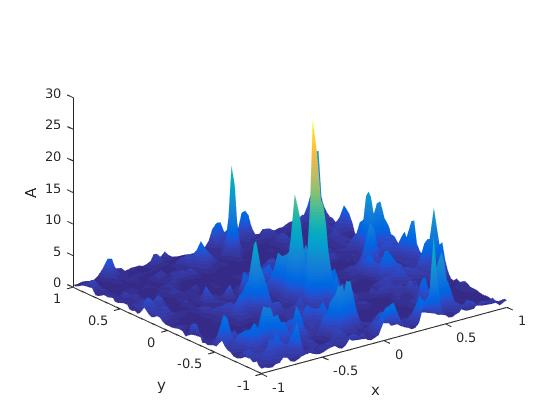
\includegraphics{Figures/A} & \includegraphics{Figures/A_zeta}
	\end{tabular}
	\caption{Estimation of the drift coefficient $A$ of \eqref{eq:SDE_HOM} with \eqref{eq:AEstDiscrete}. On both figures, the solid horizontal line is the true value of the homogenized drift coefficient $A$, while the dashed line is the value of the drift coefficient $\alpha$ of the multiscale equation. On the left, the estimation is obtained varying $\epl$ for fixed values of the coefficients $(\beta, \gamma, \zeta)$. On the right, we fix $\epl = 5\cdot 10^{-3}$, the exponent $\beta = 2$ and vary $\zeta$ and $\gamma = 2\beta - \zeta$.}
	\label{fig:A}
\end{figure} 

Let us consider the case $V_0(x) = x$ and $V_1(x) = \cos(x)$, so that the homogenized model \eqref{eq:SDE_HOM} is the Ornstein--Uhlenbeck equation. We fix $\alpha = 1$ and $\sigma = 0.5$ and wish to retrieve the drift coefficient $A$ of \eqref{eq:SDE_HOM}. In this case, the value of $K$ in \eqref{eq:K_HOM} is given by
\begin{equation}
	K = \frac{L^2}{Z\widehat Z},
\end{equation}
with $L = 2\pi$ and 
\begin{equation}
	Z = \int_0^L \exp\left(-\frac{V_1(y)}{\sigma}\right) \dd y, \quad \widehat Z = \int_0^L \exp\left(\frac{V_1(y)}{\sigma}\right) \dd y.
\end{equation}
It is therefore possible to compute cheaply the coefficients of the homogenized model and obtain a comparison for numerical results. Following Theorem \ref{thm:DriftDiscrete}, we consider a set of values of $\epl$, in particular we choose $\epl_i = 1.3^i \cdot 10^{-3}$ for $i = 0, 1, \ldots, 20$ and fix $h_i = \epl_i^\beta$ with $\beta = 2$, the averaging window $\delta_i = \epl^\zeta$ for $\zeta = \beta - 0.7$, and $N = [\epl^{-\gamma}]$ with $\gamma = 2\beta - \zeta$. Results, displayed in Figure \ref{fig:A}, show how the estimated drift coefficient tends towards the value of the homogenized coefficient. Nonetheless, given values of $\epl$ and $\beta$, the choice of $\zeta \in (\beta - 1, \beta)$ is arbitrary. Theoretically, all choices in this interval should lead asymptotically with respect to $\epl$ to the value $A$ of the homogenized equation, in law. In order to test numerically this property, we fix $\epl = 5\cdot 10^{-3}$, the exponent $\beta = 2$ and vary $\zeta$ linearly in the range $[\beta - 1, \beta]$, thus fixing $\gamma = 2\beta - \zeta$. Results, displayed in Figure \ref{fig:A}, show that the best estimations are obtained for values close to the bounds of the interval $(\beta-1, \beta)$.

We now consider inference of the diffusion coefficient $\Sigma$ of \eqref{eq:SDE_HOM}. Adopting the notation of Theorem \ref{thm:DiffDiscrete}, we first vary $\epl \in [0.01, 0.2]$ and choose $N = [\epl^{-\gamma}]$ with $\gamma = 4$. We then fix $\beta = 3$ and $\zeta = 2$. Let us remark that Theorem \ref{thm:DiffDiscrete} does only require $\gamma$ to be positive. Nonetheless, the term $I_1$ in its proof tends to $\Sigma$ for $N\to\infty$, and taking a relatively high value for $\gamma$ allows to observe convergence. Results, shown in Figure \ref{fig:S}, demonstrate the validity of the theoretical result. As for the drift coefficient, we consider the effect of varying the averaging window width, i.e., the exponent $\zeta$ such that $\delta = [\epl^{\zeta}]$. We fix $\epl = 0.02$, $\gamma = 4$ and $\beta = 3$, and vary $\zeta \in [0, \beta+1]$. For $\zeta = 0$, we retrieve the parameter $\sigma$ of the multiscale model, as it should be expected. For $\zeta > \beta$, the estimator rapidly tends to zero. The estimation appears to be correct for values of $\zeta$ in the interval $(\beta-1, \beta)$, which is the same range of validity as for the estimation of the coefficient $A$.

\begin{figure}
	\centering
	\begin{tabular}{cc}
		\includegraphics{Figures/S} & \includegraphics{Figures/S_zeta}
	\end{tabular}
	\caption{Estimation of the diffusion coefficient $\Sigma$ of \eqref{eq:SDE_HOM} with \eqref{eq:SigmaEstDiscrete}. The dashed horizontal line corresponds to the diffusion coefficient $\alpha$ of the multiscale model, while the solid line corresponds to the true homogenized value $A$. On the left, the estimation is obtained varying $\epl$ for fixed values of the coefficients $(\beta, \gamma, \zeta)$. On the right, we fix $\epl = 2\cdot 10^{-2}$, the exponents $\beta = 3$ and $\gamma = 4$ and vary $\zeta$.}
	\label{fig:S}
\end{figure}

\section{Bayesian inference}

Consider 
\begin{equation}
L_T^0(A) = \exp\left\{-\int_0^T A V_0'(X_t^0) \dd X_t^0 - \frac12 \int_0^T A^2 V_0'(X_t^0)^2 \dd t \right\},
\end{equation}
and, denoting $Z^\epl_t \defeq \mathcal H_\delta(X^\epl)_t$, where $\mathcal H_\delta$ is defined in \eqref{eq:ContMovingAverage}
\begin{equation}
L_T^\epl(A) = \exp\left\{-\int_0^T A V_0'(Z^\epl_t)\dd Z^\epl_t - \frac12 \int_0^T A^2 V_0'(Z^\epl_t)^2 \dd t \right\}.
\end{equation}
Let the prior be denoted by $\Lambda$, with density $\lambda$ and the corresponding posteriors $\mu_T^0$ and $\mu_T^\epl$. Denote $\ell_t^0 = \log L_T^0$, respectively $\ell_t^\epl$ the log-likelihoods.

Define 
\begin{equation}
d_{\mathrm{TV}}(\mu, \nu) \defeq \sup_{B \in \mathcal B} \abs{\mu(B) - \nu(B)}.
\end{equation}
Compute for $B \in \mathcal B$ 
\begin{equation}
\abs{\mu_T^0(B) - \mu_T^\epl(B)} = \abs{\frac{C^\epl \int_B L_T^0(A) \lambda(A) \dd A - Z^0 \int_B L_T^\epl(A) \lambda(A) \dd A}{C^0 C^\epl}},
\end{equation}
where
\begin{equation}
C^0 = \int_{\mathcal A} L_T^0(A) \lambda(A) \dd A,
\end{equation}
and $C^\epl$ defined respectively. Then
\begin{equation}
\abs{\mu_T^0(B) - \mu_T^\epl(B)} \leq I_1 + I_2, 
\end{equation}
where
\begin{equation}
\begin{aligned}
I_1 &= \frac{1}{C^0} \int_B \abs{L_T^0(A) - L_T^\epl(A)} \lambda(A) \dd A, \\
I_2 &= \frac{\abs{C^\epl - C^0}}{C^0 C^\epl} \mu_T^\epl(B).
\end{aligned}
\end{equation}
Consider first $I_1$. Since $\abs{\exp(a) - \exp(b)} \leq (\exp(a)+ \exp(b)) \abs{a - b}$, we have
\begin{equation}
I_1 \leq \frac{1}{C^0} \int_B \big(L_T^0(A) + L_T^\epl(A)\big)\abs{\ell_T^0(A) - \ell_T^\epl(A)} \lambda(A) \dd A.
\end{equation}
Let us consider
\begin{equation}
\begin{aligned}
\ell_T^0(A) - \ell_T^\epl(A) = &- \int_0^T A V_0'(X_t^0) \dd X_t^0 + \int_0^T A V_0'(Z^\epl_t) \dd Z^\epl_t \\
&- \frac12 \int_0^T A^2 \big(V_0'(X_t^0)^2 - V_0'(Z^\epl_t)^2\big) \dd t.
\end{aligned}
\end{equation}

\begin{lemma} Under assumptions \corr{add assumptions}, it holds
	\begin{equation}
		\abs{\ell_T^0(A) - \ell_T^\epl(A)} \to 0,
	\end{equation}
	for $\epl \to 0$.
\end{lemma}

\begin{proof} The triangle inequality
	\begin{equation}
	\begin{aligned}
		\abs{\ell_T^0(A) - \ell_T^\epl(A)} \leq &\abs{\int_0^T A V_0'(X_t^0) \dd X_t^0 - \int_0^T A V_0'(Z^\epl_t) \dd Z^\epl_t} \\
		&+ \abs{\frac12 \int_0^T A^2 \big(V_0'(X_t^0)^2 - V_0'(Z^\epl_t)^2\big) \dd t} \eqdef I_1 + I_2
	\end{aligned}
	\end{equation}
	Let us first consider $I_1$. From the definition of $Z_t^\epl$, we divide
	\begin{equation}
	\begin{aligned}
		 I_1 \leq &\abs{\int_0^\delta A V_0'(X_t^0) \dd X_t^0 - \int_0^\delta A V_0'(Z^\epl_t) \frac{X^\epl_t - Z^\epl_t}{t}\dd t}\\
		 + &\abs{\int_\delta^T A V_0'(X_t^0) \dd X_t^0 - \int_\delta^T A V_0'(Z^\epl_t) \frac{X^\epl_t - X^\epl_{t-\delta}}{\delta}\dd t} \eqdef I_1^1 + I_1^2.
	\end{aligned} 
	\end{equation}
	Let us first consider $I_1^2$. Replacing \eqref{eq:ContDiffDecomp} we can write in law
	\begin{equation}
		I_1^2 = \abs{\int_\delta^T A V_0'(X_t^0) \dd X_t^0 - \int_\delta^T A V_0'(Z^\epl_t) \frac{J_t - A\delta V_0'(Z_t^\epl) + R(\epl, \delta)}{\delta}\dd t},
	\end{equation}
	where, due to Lemma \ref{lem:ContFirstBound}, we have
	\begin{equation}
		\left( \E^{\mu^\epl} \abs{R(\epl, \delta)}^p \right)^{1/p} \leq C(\epl^2 + \delta^{1/2} + \delta^{3/2}).
	\end{equation}
	Replacing $\d X^0_t$ with its definition given by \eqref{eq:SDE_HOM}, we can then split $I_1^2$ in three terms and apply the triangle inequality as
	\begin{equation}
	\begin{aligned}
		I_1^2 &\leq A^2 \abs{\int_\delta^T  \left(V_0'(X_t^0)^2 - V_0'(Z_t^\epl)^2\right) \dd t} + A \abs{\int_\delta^T  V_0'(X^0_t)\sqrt{2\Sigma}\dd W_t - \frac{1}{\delta} \int_\delta^T V_0'(Z_t^\epl) J_t \dd t} \\
		&\quad+ A \abs{\int_\delta^T V_0'(Z_t^\epl) \frac{R(\epl, \delta)}{\delta}\dd t} \eqdef R_1 + R_2 + R_3.
	\end{aligned}
	\end{equation}	
\end{proof}

%We now need a decomposition similar to \eqref{eq:ContDiffDecomp} for the process $Z^\epl_t$. A first step is given by the following lemma.
%\begin{lemma}\label{lem:ReprMovAv} The process $Z^\epl_t \defeq \mathcal H_\delta(X^\epl_t)$, where $\mathcal H_\delta$ is defined in \eqref{eq:ContMovingAverage}, admits for $\delta \leq t \leq T$ the representation
%	\begin{equation}
%	Z^\epl_t =  X^\epl_{t-\delta} - \frac1\delta\int_{t-\delta}^{t} (t - s) \left( \alpha V_0'(X^\epl_s) + \frac1\epl V_1'\left(Y_s^\epl\right)\right) \dd s + \frac1\delta \int_{t-\delta}^{t} \sqrt{2\sigma} (t-s) \dd W_s,
%	\end{equation}
%	where $(X_t^\epl, Y_t^\epl)$ is the solution of \eqref{eq:SDE_MS2}.
%\end{lemma} 
%\begin{proof}
%	Let us for ease of notation denote $Z_t \defeq Z^\epl_t$, $X_t \defeq X^\epl_t$ and 
%	\begin{equation}
%	f(X_t) \defeq -\alpha V_0(X_t) - \frac1\epl V_1\left(Y_t^\epl\right).
%	\end{equation}
%	Due to the definition of $Z_t$, we have
%	\begin{equation}\label{eq:ReprStart}
%	\delta Z_t = \delta X_{t-\delta} + \int_{t-\delta}^{t}\int_{t-\delta}^s f(X_r) \dd r\dd s + \int_{t-\delta}^{t}\int_{t-\delta}^s \sqrt{2\sigma}\dd W_r \dd s,
%	\end{equation}
%	where, exchanging the order of integration, we obtain for the deterministic integral
%	\begin{equation}\label{eq:ReprDet}
%	\begin{aligned}
%	\int_{t-\delta}^{t}\int_{t-\delta}^s f(X_r) \dd r\dd s &= \int_{t-\delta}^{t}\int_r^t f(X_r) \dd s \dd r\\
%	&= \int_{t-\delta}^{t} (t - s) f(X_s) \dd s.
%	\end{aligned}
%	\end{equation}
%	For the stochastic integral, we can write
%	\begin{equation}
%	\begin{aligned}
%	\int_{t-\delta}^{t}\int_{t-\delta}^s \dd W_r \dd s &= \int_{t-\delta}^{t} (W_s - W_{t-\delta}) \dd s \\
%	&= \int_{t-\delta}^{t} W_s \dd s - \delta W_{t-\delta}.
%	\end{aligned}
%	\end{equation}
%	The formula $\d(tW_t) = t\dd W_t + W_t \dd t$ yields
%	\begin{equation}
%	\begin{aligned}
%	\int_{t-\delta}^{t} W_s \dd s &= \big(tW_t - (t-\delta) W_{t-\delta}\big) - \int_{t-\delta}^{t} s \dd W_s\\
%	&=  t(W_t - W_{t-\delta}) - \int_{t-\delta}^{t} s \dd W_s + \delta W_{t-\delta}\\
%	&= \int_{t-\delta}^{t} (t-s) \dd W_s + \delta  W_{t-\delta},
%	\end{aligned}
%	\end{equation}
%	which implies
%	\begin{equation}\label{eq:ReprStoch}
%	\int_{t-\delta}^{t}\int_{t-\delta}^s \dd W_r \dd s = \int_{t-\delta}^{t} (t-s) \dd W_s.
%	\end{equation}
%	Replacing \eqref{eq:ReprDet} and \eqref{eq:ReprStoch} into \eqref{eq:ReprStart} then gives the desired result.
%\end{proof}

\bibliographystyle{siam}
\bibliography{../../anmc}
\end{document}  